\subsection{Translator Components}

Translator runs as a separate component independent on existing GitHub infrastructure. Translator is responsible for:
\begin{itemize}
  \item Translating existing Git Commits to Subersion revisions
  \item Processing of Subversion user's requests
  \item Translating new Subersion revisions to Git commits
  \item Pushing translated Git commits to GitHub Git repository
\end{itemize}
Translator components are depicted on the diagram \ref{translator_components_pic}:
\begin{figure}[!h]
\label{translator_components_pic}
\centering
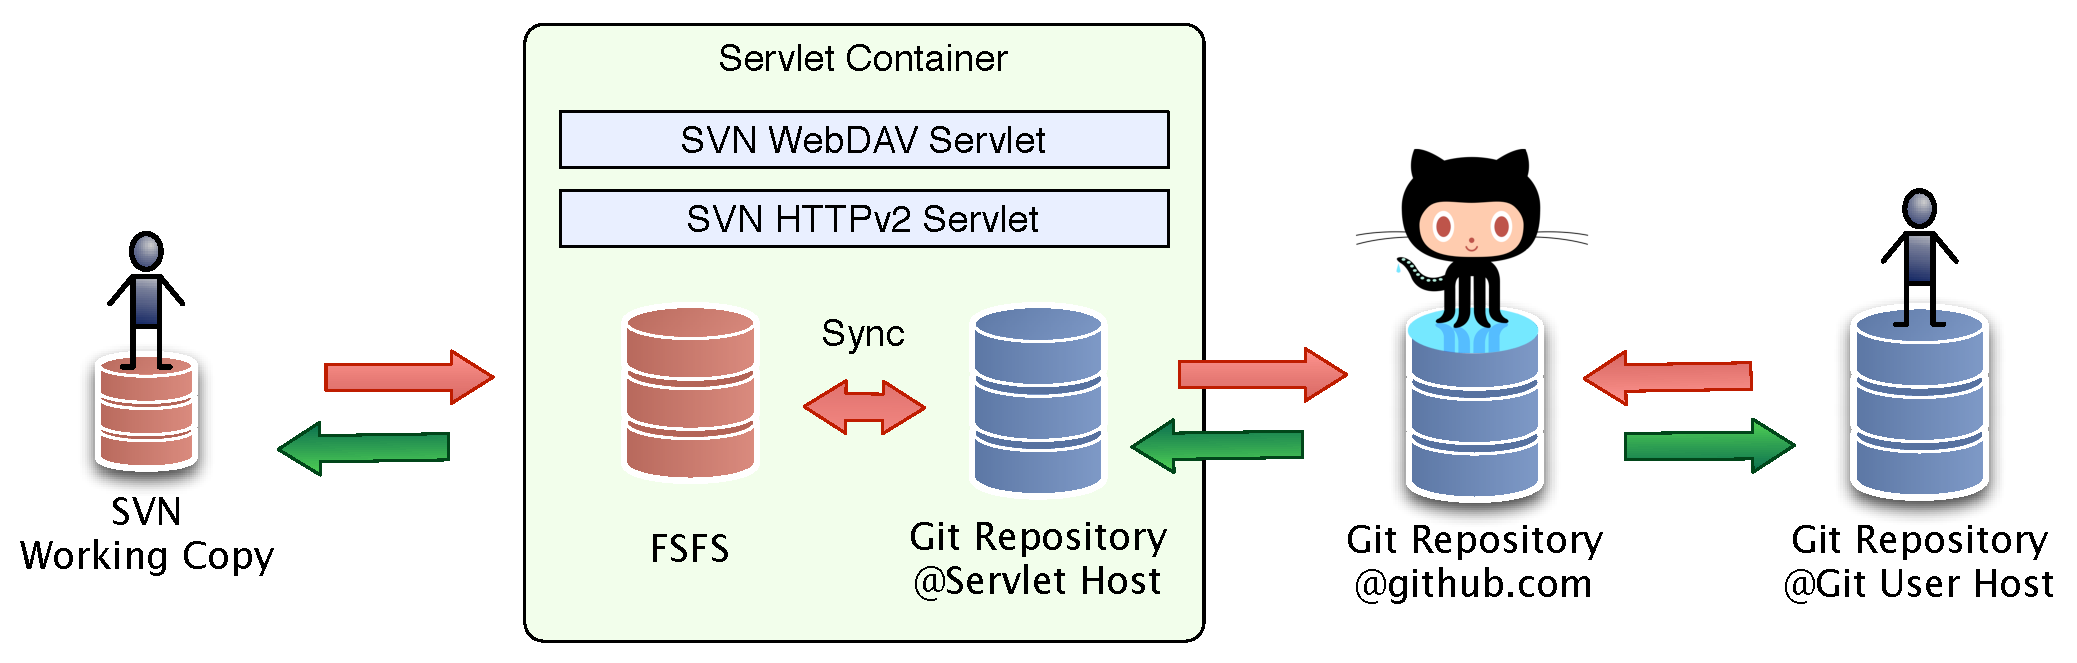
\includegraphics[width=\linewidth]{img/servlet/components_keep_github_safe.pdf}
\caption{Translator Components}
\end{figure}

Translator major features from the architecture perspective are \emph{maximum level of reuse} of the standard existing components, and \emph{minimum interference} with the existing GitHub infrastructure. 
Let's take a look at how these features are implemented. This chapter provides an overview of Translator components and further chapters provides more details on how each particular operation is carried on.

\label{srp}
\subsubsection{Subversion Requests Processor}
In order to process Subversion user's requests sent over HTTP protocol, Translator is implemented as a Java servlet which might be ran inside any servlet container. All Subversion requests are served by the standard Subversion processing code which serves 
these request by reading from or writing to the local Subversion repository (see FSFS at figure \ref{translator_components_pic}).
\\\\
Processing some of the write requests includes calls to \emph{hooks} which instantly translates Subversion revisions to Git commits.
\\\\
\textbf{Reused:} existing Subversion codebase; Subversion repository as a data storage.\\
\textbf{Interference with GitHub infrastructure:} none. 

\subsubsection{Git to Subversion Translator}
To make any sense, local Subversion repository must be kept up to date with its GitHub counterpart, i.e. it have to include all the changes committed into GitHub repository by Git users. Synchronization of the local Subversion repository with GitHub Git repository is performed in two steps:
\begin{enumerate}
\item Changes in GitHub Git repository are pulled to the local Git repository
\item Git commits from local Git repository are imported into the local Subversion repository
\end{enumerate} 
Synchronization takes place:
\begin{itemize}
\item Before Subversion repository becomes available to the users, to import existing Git commits into Subversion repository
\item Just before Subverion commit is translated into Git commit to make sure Subversion repository is up to date
\item On schedule, to minimize delays on commit
\end{itemize} 
Import of Git commits into Subversion repository is performed with the help of SVNGitKit Java library.
\\\\
\textbf{Reused:} SVNGitKit library to import commits; Git code to clone and fetch from GitHub Git repository into the local one.\\
\textbf{Interference with GitHub infrastructure:} similar to other GitHub clients, this component of Translator clones and then fetches new changes into its clone of GitHub repository.

\subsubsection{Subversion to Git Translator}
Commits made by Subversion users are instantly translated into Git commits which are then pushed into GitHub Git repository. Component repsonsible 
for that instant translation and push is implemeted as \emph{hooks} called by Subversion code during commit (see \ref{srp}).
\newpage 
This approach helps to make sure that Subversion commit and corresponding Git push operation are part of the same transaction and either succeeds or fails together.
For more detailed description of how Subversion commits are processed, refer to the section 1.2 of this specification.
\\\\
\textbf{Reused:} Instant translation uses SVNGitKit library, small part of the code is custom, in particular part which is responsible for integrity of Subversion commit and Git push pair.\\
\textbf{Interference with GitHub infrastructure:} similar to other GitHub clients, this component of Translator peformes push of the new Git objects into GitHub Git repository.

\subsubsection{GitHub Integration}

Translator architecture minimizes interference with the existing GitHub infrastructure which is clearly an advantage, but there is a performance penalty being paid for that.
In particular, there is sychronization of the local Git repository with the GitHub Git repository using fetch and push operations. Moreover, both fetch and push are 
performed as part of Subversion commit operation, which might make Subversion commits slow and prone to timeout related errors.
\\\\
To resolve this potential performance issue, Translator could benefit from having local filesystem access to the GitHub repository. Then Translator may work directly with GitHub repository,
with no need to use expensive push and fetch operations.
\begin{figure}[!h]
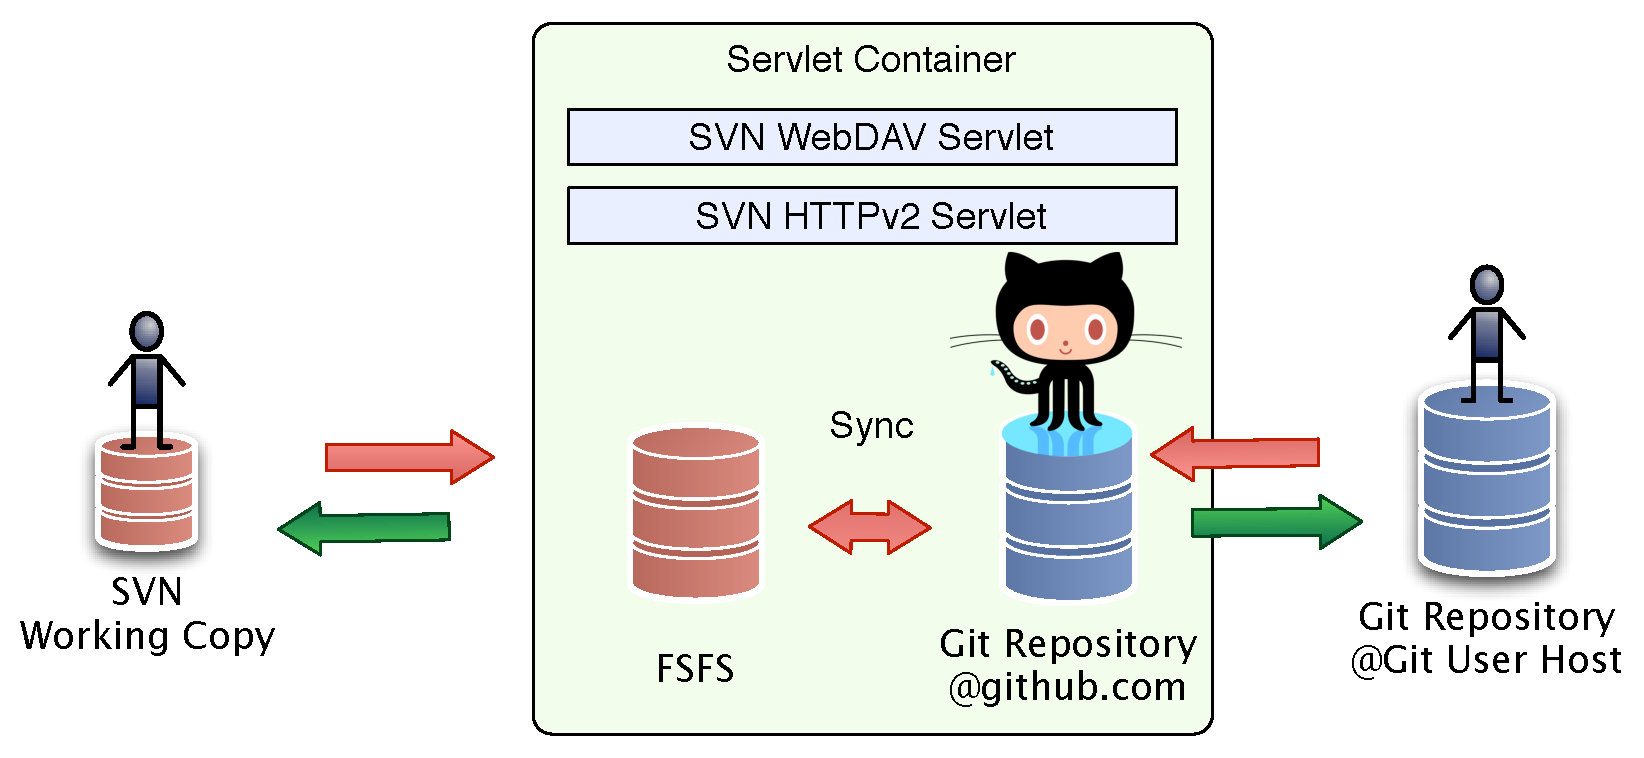
\includegraphics[width=\linewidth]{img/servlet/components_not_that_safe.pdf}
\caption{Higher level of interference}
\label{translator_components_pic2}
\end{figure}
Major drawback of that solution is that theoretically, bug in Translator code may damage existing GitHub repository contents.